\documentclass[12pt, oneside]{article}

%Codificación e idioma
\usepackage[T1]{fontenc}
\usepackage[spanish]{babel}
\usepackage[utf8]{inputenc}

% Url
\usepackage{url}

% Graphics
\usepackage[pdftex]{graphicx}
\DeclareGraphicsExtensions{.png,.jpg}

\usepackage{wrapfig}

%Resaltado de sintaxis
\usepackage{color}
\definecolor{gray97}{gray}{.97}
\definecolor{gray75}{gray}{.75}
\definecolor{gray45}{gray}{.45}

\definecolor{red}{rgb}{0.6,0,0} % strings
\definecolor{green}{rgb}{0.25,0.5,0.35} % comments
\definecolor{purple}{rgb}{0.5,0,0.35} % keywords
\definecolor{blue}{rgb}{0.25,0.35,0.75} % doc

\usepackage{listings}
\lstset {
	language			=	C,
	frame				=	Ltb,
    framerule			=	0pt,
    aboveskip			=	0.5cm,
    framextopmargin		=	3pt,
    framexbottommargin	=	3pt,
    framexleftmargin	=	0.4cm,
    framesep			=	0pt,
    rulesep				=	.4pt,
    backgroundcolor		=	\color{gray97},
    rulesepcolor		=	\color{black},
    %
    stringstyle			=	\color{red},
    showstringspaces	=	false,
    basicstyle			=	\ttfamily\small,
    commentstyle		=	\color{green},
    morecomment         =   [s][\color{blue}]{/*}{*/},
    keywordstyle		=	\color{purple}\bfseries,
    tabsize					=	3,
    %
    numbers				=	left,
    numbersep			=	15pt,
    numberstyle			=	\tiny,
    numberfirstline		=	false,
    breaklines			=	true,
}

\title{Apache Torque}
\author{Francisco J. Serrano}

\begin{document}

\maketitle
\tableofcontents

\section{Introducción}

\subsection{Fundación Apache}

\begin{wrapfigure}{L}{0.3\textwidth}
	
\includegraphics[scale=.8]{img/apache-logo.png}
\end{wrapfigure}

Apache Software Foundation (ASF) es una organización no lucrativa (en concreto, una fundación) creada para dar soporte a los proyectos de software bajo la denominación Apache, incluyendo el popular servidor HTTP Apache. La ASF se formó a partir del llamado Grupo Apache y fue registrada en Delaware (Estados Unidos), en junio de 1999.
Apache Software Foundation es una comunidad descentralizada de desarrolladores que trabajan cada uno en sus propios proyectos de código abierto. Los proyectos Apache se caracterizan por un modelo de desarrollo basado en el consenso y la colaboración y en una licencia de software abierta y pragmática.

\subsection{Apache Torque}

\begin{wrapfigure}{L}{0.4\textwidth}
	
\includegraphics[scale=.8]{img/torque-logo.png}
\end{wrapfigure}

Apache Torque es un mapeador objeto relacional para Java. En otras palabras, Torque te permite acceder y manipular información en una base de datos relacional usando objetos. 
%A diferencia de la mayoría de los otros mapeadores objeto-relacional, Torque no utiliza la reflexión para tener acceso a las clases proporcionadas por el usuario, pero genera las clases necesarias (incluyendo los Objetos) a partir de un esquema XML que describe el diseño de base de datos (que puede ser escrito a mano o generado a partir de una base de datos existente)
El esquema XML puede ser usado para generar y ejecutar un script SQL el cual creará todas la tablas en la base de datos.

As Torque hides database-specific implementation details, Torque makes an application independent of a specific database if no exotic features of the database are used.
Usage of autogeneration eases the customization of the database layer, as you can override the autogenerated methods and thus easily change their behaviour.

\subsubsection{Runtime}
Torque Runtime contiene todo lo necesario para permitir a la aplicación acceder a la base de datos. Es el único componente que Torque necesita en la aplicación y puede ser usado de forma independiente.

\subsubsection{Generator}
Generator contiene las tareas de Ant las cuales hacen todo el trabajo para el plugin Maven. En el caso de usar el plugin Maven, no es necesario usar Generator directamente. No obstante, Generator puede ser llamado directamente desde Ant.

\subsubsection{Ant}

\begin{wrapfigure}{L}{0.3\textwidth}
	
\includegraphics[scale=.9]{img/ant-logo.png}
\end{wrapfigure}

Apache Ant es una libreria de Java y una herramienta de linea de comando cuya misión es
Apache Ant is a Java library and command-line tool whose mission is to drive processes described in build files as targets and extension points dependent upon each other. The main known usage of Ant is the build of Java applications. Ant supplies a number of built-in tasks allowing to compile, assemble, test and run Java applications. Ant can also be used effectively to build non Java applications, for instance C or C++ applications. More generally, Ant can be used to pilot any type of process which can be described in terms of targets and tasks. Ant is written in Java. Users of Ant can develop their own "antlibs" containing Ant tasks and types, and are offered a large number of ready-made commercial or open-source "antlibs". Ant is extremely flexible and does not impose coding conventions or directory layouts to the Java projects which adopt it as a build tool.

\subsubsection{Maven Plugin}

\begin{wrapfigure}{L}{0.3\textwidth}
	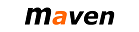
\includegraphics[scale=.8]{img/maven-logo.png}
\end{wrapfigure}

Maven plugin: Apache Maven is a software project management and comprehension tool. Based on the concept of a project object model (POM), Maven can manage a project's build, reporting and documentation from a central piece of information. (Nosotros no lo usaremos)

\subsubsection{Templates}
The templates contain the building blocks used by the generator to create the O/R peer and object classes, SQL scripts and the like. You can change the templates if you want to customize the output of the generator (this is only necessary in very special circumstances). Up to release 3.1.x, the templates were a part of the generator. Starting with the 3.2 release of Torque, the templates have been separated into their own jar archive.

\subsubsection{Village}
Village is a 100\% Pure Java API that sits on top of the JDBC API. El propósito de esta API es hacer mas fácil is to make it easier to interact with a JDBC compliant relational database.

\section{Gestores de bases de datos}

\subsection{Postgresql}

\begin{wrapfigure}{L}{0.3\textwidth}
	
\includegraphics[scale=.8]{img/postgresql-logo.png}
\end{wrapfigure}

PostgreSQL es un sistema de gestión de bases de datos objeto-relacional, distribuido bajo licencia BSD y con su código fuente disponible libremente. Es el sistema de gestión de bases de datos de código abierto más potente del mercado.
PostgreSQL utiliza un modelo cliente/servidor y usa multiprocesos en vez de multihilos para garantizar la estabilidad del sistema. Un fallo en uno de los procesos no afectará el resto y el sistema continuará funcionando.

\subsection{MySQL}

\begin{wrapfigure}{L}{0.35\textwidth}
	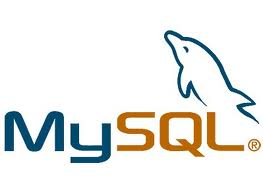
\includegraphics[scale=.3]{img/mysql-logo.jpg}
\end{wrapfigure}

MySQL es un sistema de gestión de base de datos relacional cuya licencia se ofrece bajo GNU GPL.
MySQL usa un sistema multihilo y funciona sobre una gran cantidad de plataformas.
En aplicaciones web hay baja concurrencia en la modificación de datos y en cambio el entorno es intensivo en lectura de datos, lo que hace a MySQL ideal para este tipo de aplicaciones gracias a su motor no transaccional MyISAM.

\subsection{SQL Server}

\section{Instalando Apache Torque}
En primer lugar descargar todo el software necesario:

\begin{description}
	\item[Runtime] \url{http://apache.rediris.es/db/torque/torque-3.3/binaries/torque-3.3.tar.gz}
	\item[Generator] \url{http://ftp.udc.es/apache/db/torque/torque-3.3/binaries/torque-gen-3.3.tar.gz}
	\item[Village] \url{http://apache.rediris.es/db/torque/torque-3.3/binaries/village-3.3.tar.gz}
	\item[Ant] \url{http://ftp.udc.es/apache//ant/binaries/apache-ant-1.8.4-bin.zip}
\end{description}

\subsection{Instalando Ant}
Después de descargar Ant, lo descomprimimos en nuestro directorio C: por ejemplo.
Renombramos la carpeta descomprimida “apache-ant-1.8.4” como “ant”.
Ejecutamos cmd.exe e introducimos las siguientes variables de entorno:

\begin{lstlisting}
ANT_HOME: set ANT_HOME= C:\ant
JAVA_HOME: set JAVA_HOME C:\Program Files\Java\jdk1.7.0_07 (Directorio donde se encuentra vuestra maquina JAVA)
\end{lstlisting}

Introducimos la dirección del directorio “ant” en el PATH:
\begin{lstlisting}
set PATH=%PATH%;%ANT_HOME%\bin
\end{lstlisting}

Obtenemos las dependencias de bibliotecas de Ant:

Desde cmd.exe nos dirigimos al directorio de Ant
Dentro de él ejecutamos los siguiente:  ant -f fetch.xml -Ddest=system

Instalación de Ant finalizada, ya podemos usar Ant desde cmd.exe.

\subsection{Creando un proyecto}
Creamos un nuevo proyecto en eclipse.
En el interior de la carpeta del proyecto descomprimimos los siguientes paquetes: runtime, generator y village.

\subsection{Configurando y ejecutando Generator}
Accedemos a la carpeta “torque-gen-3.3” de nuestro proyecto.

Descargamos el driver JDBC de la base de datos que queremos utilizar, en nuestro caso Postgresql, desde la siguiente dirección: http://jdbc.postgresql.org/ y lo introducimos en la carpeta “lib” de Generator.

En Postgresql, creamos un usuario “user1” con contraseña “user1” y una base de datos llamada “coches”, de la que es propietario “user1”.

Creamos un directorio en la raíz del proyecto llamado “schema”, donde introduciremos el archivo xml en el cual se describe la base de datos.

Editamos el archivo “build.propierties” añadiendo la configuración de nuestro proyecto. En amarillo se encuentran las líneas que han sido modificadas con respecto al archivo de configuración por defecto.

\subsubsection{build.propierties}
El fichero {\bf build.propierties} es un extenso fichero en texto plano estructurado en apartados.

A continuación verá las lineas que han sido necesarias modificar para que el ejemplo {\em coches} funcione correctamente.

En el apartado {\bf PROYECT}, se ha modificado el nombre de proyecto. {\bf Apache Torque} usará {\em el nombre de proyecto} como base tanto para buscar el fichero xml así como nombre base para generar archivos del proyecto.
\begin{lstlisting}
# Nombre de nuestro proyecto
torque.project = coches
\end{lstlisting}

En el apartado {\bf TARGET DATABASE} buscaremos una línea para asignar como valor el nombre de la base de datos que deseemos utilizar. Las opciones disponibles son:

\begin{multicols}{2}
\begin{itemize}
	\item axion
	\item cloudscape
	\item db2
	\item db2400
	\item hypersonic
	\item interbase
	\item msaccess
	\item mssql
	\item mysql
	\item oracle
	\item postgresql
	\item sapdb
	\item sybase
\end{itemize}
\end{multicols}

En nuestro ejemplo usuaremos {\bf PostgreSQL}, por lo que la variable quedaría definida:
\begin{lstlisting}
# Gestor de bases de datos que vamos a usar
torque.database = postgresql
\end{lstlisting}

En el apartado {\bf DATABASE SETTINGS}, configuraremos las opciones de conexión del JDBC. Estos datos son usados por {\bf Ant} para inicializar el sistema Torque con el SQL generado.
\begin{lstlisting}
# Direcciones de acceso a la base de datos y puerto de escucha
torque.database.createUrl = jdbc:postgresql://127.0.0.1:5432/coches
torque.database.buildUrl = jdbc:postgresql://127.0.0.1:5432/coches
torque.database.url = jdbc:postgresql://127.0.0.1:5432/coches

# Driver para acceder a la base de datos
torque.database.driver = org.postgresql.Driver

# Usuario y password para acceder a la base de datos
torque.database.user = user1
torque.database.password = user1

#Direccion del host donde se encuentra la base de datos
torque.database.host = 127.0.0.1

# Direccion donde se generaran los ficheros .java y .sql
torque.output.dir = ../src

# Direccion desde donde se obtendra el esquema .xml de la base de datos
torque.schema.dir = ../schema
\end{lstlisting}

Ahora creamos un archivo XML llamado "coches-schema.xml", en el directorio "schema", donde describiremos la estructura de la base de datos de nuestro sistema. (En este ejemplo solo se usará una tabla, más adelante se explicará las diferentes configuraciones de este fichero)

subsubsection{coches-schema.xml}
Ahora creamos un archivo XML llamado {\bf coches-schema.xml}, en el directorio {\bf schema}, donde describiremos la estructura de la base de datos de nuestro sistema.
{\em En este ejemplo solo se usará una tabla, más adelante se explicará las diferentes configuraciones de este fichero. La tabla usada es la siguiente:}

\begin{lstlisting}[language=xml]
<!DOCTYPE database SYSTEM "http://db.apache.org/torque/dtd/database_3_3.dtd">

<database name="coches">
	<table name="coche" description="Tabla de coches">
	<column
		name="coche_id"
		required="true"
		primaryKey="true"
		type="INTEGER"
		description="Identificador de coches"/>
	<column
		name="nombre"
		required="true"
		type="VARCHAR"
		size="128"
		description="Nombre del coche"/>
	</table>
</database>
\end{lstlisting}

Desde cmd.exe accedemos al directorio {\bf torque-gen-3.3} y ejecutamos las siguientes instrucciones:
\begin{enumerate}
	\item Esta instrucción genera los archivos .java y .sql en la carpeta que hemos indicado antes en nuestro archivo {\em build.propierties}, en nuestro caso en {\em src}:
	\begin{lstlisting}
	ant -f build-torque.xml
	\end{lstlisting}
	 
	\item La siguiente crea y configura la base de datos:
	\begin{lstlisting}
	ant -f build-torque.xml create-db
	\end{lstlisting}
	
	\item Por último esta instrucción crea las tablas en la base de datos, ejecutando el .sql creado con anterioridad: 
	\begin{lstlisting}
	ant -f build-torque.xml insert-sql
	\end{lstlisting}
\end{enumerate}

Ya tenemos en la carpeta {\em src} dos subcarpetas, una llamada {\em java} donde se encuentran los fuentes de nuestro proyecto; y otra llamada {\em sql}, donde se encuentran los scripts de generación de la base de datos. Movemos la carpeta {\em sql} a la raíz del proyecto, ya que no la necesitaremos.

Finalmente movemos el contenido del directorio {\em java} al directorio {\em src} y eliminamos el directorio {\em java}. Ya tenemos el proyecto preparado, para seguir trabajando desde Eclipse.

Desde cmd.exe accedemos al directorio “torque-gen-3.3” y ejecutamos las siguientes instrucciones: 
Esta instrucción genera los archivos .java y .sql en la carpeta que hemos indicado antes en nuestro archivo “build.propierties”, en nuestro caso en “src”: ant -f build-torque.xml 
La siguiente crea y configura la base de datos:  ant -f build-torque.xml create-db.
Por último esta instrucción crea las tablas en la base de datos, ejecutando el .sql creado con anterioridad: ant -f build-torque.xml insert-sql

Ya tenemos en la carpeta “src” 2 subcarpetas, una llamada “java” donde se encuentran los fuentes de nuestro proyecto y otra llamada “sql”, donde se encuentran los scripts de generación de la base de datos. Movemos la carpeta sql a la raíz del proyecto, ya que no la necesitaremos. Finalmente movemos el contenido del directorio “java” al directorio “src” y eliminamos el directorio “java”. Ya tenemos el proyecto preparado, para seguir trabajando desde Eclipse.

\subsection{Configuración del proyecto desde Eclipse}
Como podemos observar existen numerosos errores en nuestro proyecto, ello es debido a la falta de las librerías de Torque y Village. Las añadimos desde las siguientes direcciones:

\begin{lstlisting}
coches\torque-3.3\lib
\end{lstlisting}

	\begin{center}
		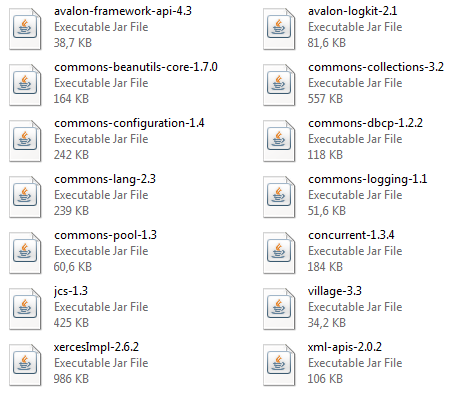
\includegraphics[height=8cm]{img/torque-lib.png}
	\end{center}
	
\begin{lstlisting}
coches\torque-3.3\
\end{lstlisting}

	\begin{center}
		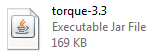
\includegraphics{img/torque-file.png}
	\end{center}
	
	Ahora ya no existen errores en el proyecto y podemos realizar una pequeña prueba de ejecución, para ello podemos crear un paquete, donde crearemos una clase Main e introduciremos el siguiente código:
	
	\begin{lstlisting}[language=java]
import java.util.Iterator;
import java.util.List;

import org.apache.torque.Torque;
import org.apache.torque.TorqueException;
import org.apache.torque.util.Criteria;

import torque.generated.Coche;
import torque.generated.CochePeer;

public class Main 
{
	public static void main(String[] args)
	{
		/*Aqui inicializamos Torque*/
		try
		{
			Torque.init("Torque.properties");
		} 
		catch (TorqueException e) 
		{	
			e.printStackTrace();
		}
		/*Aqui probamos la conexion con la base de datos*/
		try 
		{
			Coche c = new Coche();
			c.setCocheId(3);
			c.setNombre("mondeo");
			c.save();

			Coche c1 = new Coche();
			c1.setCocheId(4);
			c1.setNombre("jumpy");
			c1.save();

		} 
		catch (Exception e) 
		{
			e.printStackTrace();
		}

		/*Aqui recuperamos los datos y los mostramos por pantalla*/
		try 
		{
			Criteria crit = new Criteria();

			List<Coche> coches = CochePeer.doSelect(crit);
			for (Iterator<Coche> i = coches.iterator(); i.hasNext();)
			{
				Coche c = (Coche) i.next();
				System.out.println("coche_id: " + c.getCocheId());
				System.out.println("nombre:  " + c.getNombre()); 
				System.out.println();
			}
		} 
		catch (TorqueException e) 
		{
			e.printStackTrace();
		}
	}
}
\end{lstlisting}
	
	Desde nuestro main debemos de inicializar Torque, para ello hemos insertado la línea de código: Torque.init("Torque.properties"). Toque.init toma como parámetro un fichero llamado Torque.properties, situado en la carpeta “torque-3.3”. Movemos ese archivo a la raíz del proyecto (para que sea accesible directamente), y procedemos a configurarlo. En amarillo se encuentran las líneas que han sido modificadas con respecto al archivo de configuración por defecto.
	
	\begin{lstlisting}
# Licensed to the Apache Software Foundation (ASF) under one
# or more contributor license agreements.  See the NOTICE file
# distributed with this work for additional information
# regarding copyright ownership.  The ASF licenses this file
# to you under the Apache License, Version 2.0 (the
# "License"); you may not use this file except in compliance
# with the License.  You may obtain a copy of the License at
#
#   http://www.apache.org/licenses/LICENSE-2.0
#
# Unless required by applicable law or agreed to in writing,
# software distributed under the License is distributed on an
# "AS IS" BASIS, WITHOUT WARRANTIES OR CONDITIONS OF ANY
# KIND, either express or implied.  See the License for the
# specific language governing permissions and limitations
# under the License.

# Directorio del proyecto
torque.applicationRoot = .

# ###########
#
#  L O G G I N G
#
# ###########
# We use Log4J for all Torque logging and we embed the log4j
# properties within our application configuration.
# ###########

# This first category is required and the category
# must be named 'default'. This is used for all logging
# where an explicit category is not specified.

# Configuraciones de logging
log4j.category.org.apache.torque = ALL, org.apache.torque
log4j.appender.org.apache.torque = org.apache.log4j.FileAppender
log4j.appender.org.apache.torque.file = ${torque.applicationRoot}/logs/torque.log
log4j.appender.org.apache.torque.layout = org.apache.log4j.PatternLayout
log4j.appender.org.apache.torque.layout.conversionPattern = %d [%t] %-5p %c - %m%n
log4j.appender.org.apache.torque.append = false

# ###########
#
#  D E F A U L T S
#
# ###########
#
# These values kick in, if you don't explicitly override them in your
# various database settings. At the moment they're only used if you
# configure the SharedPoolDataSourceFactory of the PerUserDataSourceFactory
# as your data source provider. It does not work with JNDI.
#
# The example is shown for SharedPoolDataSource.
#
# ###########

# Time to wait for a connection to the database in milliseconds.
torque.defaults.pool.maxWait = 10000

# Maximum number of idle and active connections cached in a database
# definition.
# Note that, if you have multiple database definitions which access the
# same database URL, they don't share the connections but you have
# multiple pools and each has this maximum number. So if you have a
# connection licensed database engine, you must multiply this number by
# the number of times you use a specific database URL.

torque.defaults.pool.maxIdle = 8
torque.defaults.pool.maxActive = 10

# How often the pool is checked for connection which stayed in the pool
# for too long. Defaults to 5 minutes (5 * 60 * 1000)
# remove property if the idle object evictor should not be run

torque.defaults.pool.timeBetweenEvictionRunsMillis= 300000

# Lifetime of an idle connection in the pool in milliseconds.
# Defaults to one hour (1000 * 60 * 60)

torque.defaults.pool.minEvictableIdleTimeMillis = 3600000

# Sets the driver for the data sources.
# Driver de la base de datos
torque.defaults.connection.driver = org.postgresql.Driver

# Sets the URL for the datasources

# URL de la base de datos
torque.defaults.connection.url = jdbc:postgresql://127.0.0.1:5432/coches

# Sets login and password for the data sources.

# Usuario y password para acceder a la base de datos coches
torque.defaults.connection.user = user1
torque.defaults.connection.password = user1

# ###########
#
#  T O R Q U E  P R O P E R T I E S
#
# ###########
# These are your database settings. Look in the
# org.apache.torque.pool.* packages for more information.
#
# The parameters to connect to the default database.  You MUST
# configure these properly.
# ###########

# Nombre de la base de datos
torque.database.default=coches

# Gestor de base de datos
torque.database.coches.adapter=postgresql

# # Using commons-dbcp
torque.dsfactory.coches.factory=org.apache.torque.dsfactory.SharedPoolDataSourceFactory
# torque.dsfactory.coches.factory=org.apache.torque.dsfactory.PerUserPoolDataSourceFactory
torque.dsfactory.coches.pool.maxIdle=8
torque.dsfactory.coches.pool.maxActive=10
torque.dsfactory.coches.pool.testOnBorrow=true
torque.dsfactory.coches.pool.validationQuery=SELECT 1
torque.dsfactory.coches.connection.driver = org.postgresql.Driver
torque.dsfactory.coches.connection.url = jdbc:postgresql://127.0.0.1:5432/coches
torque.dsfactory.coches.connection.user = user1
torque.dsfactory.coches.connection.password = user1

# # Using jndi
# torque.dsfactory.coches.factory=org.apache.torque.dsfactory.JndiDataSourceFactory
# torque.dsfactory.coches.jndi.path=jdbc/coches
# torque.dsfactory.coches.jndi.java.naming.factory.initial = org.apache.naming.java.javaURLContextFactory
# torque.dsfactory.coches.jndi.java.naming.factory.url.pkgs = org.apache.naming

# torque.dsfactory.coches.datasource.dataSourceName=jdbc/DBcoches
# torque.dsfactory.coches.datasource.jndiEnvironment.java.naming.factory.initial = org.apache.naming.java.javaURLContextFactory
# torque.dsfactory.coches.datasource.jndiEnvironment.java.naming.factory.url.pkgs = org.apache.naming
# torque.dsfactory.coches.datasource.maxIdle=8
# torque.dsfactory.coches.datasource.maxActive=10

# # ConnectionPoolDataSource
# torque.dsfactory.coches.factory=org.apache.torque.dsfactory.JndiDataSourceFactory
# torque.dsfactory.coches.jndi.path=jdbc/DBcoches
# torque.dsfactory.coches.jndi.java.naming.factory.initial = org.apache.naming.java.javaURLContextFactory
# torque.dsfactory.coches.jndi.java.naming.factory.url.pkgs = org.apache.naming
# torque.dsfactory.coches.datasource.classname=org.apache.commons.dbcp.cpdsadapter.DriverAdapterCPDS
# torque.dsfactory.coches.datasource.driver = org.gjt.mm.mysql.Driver
# torque.dsfactory.coches.datasource.url = jdbc:mysql://localhost:3306/torque
# torque.dsfactory.coches.datasource.user = user
# torque.dsfactory.coches.datasource.password = password

# Determines if the quantity column of the IDBroker's id_table should
# be increased automatically if requests for ids reaches a high
# volume.

torque.idbroker.clever.quantity=true

# Determines whether the managers cache instances of the business objects.
# And also whether the MethodResultCache will really cache results.

torque.manager.useCache = true
\end{lstlisting}
	
	Como último paso añadimos el driver de la base de datos a nuestro proyecto en Eclipse, situado en:
	
\begin{lstlisting}
coches\torque-gen-3.3\lib
\end{lstlisting}

	\begin{center}
		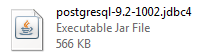
\includegraphics{img/postgresql-file.png}
	\end{center}

	Ya finalmente podemos ejecutar el proyecto, la salida por pantalla sería la siguiente: 
	
	\begin{lstlisting}
	coche_id: 3
	nombre:  mondeo

	coche_id: 4
	nombre:  jumpy
	\end{lstlisting}

\subsection{Compilando nuestro primer proyecto}
\subsection{Configuración XML}
	\begin{center}
		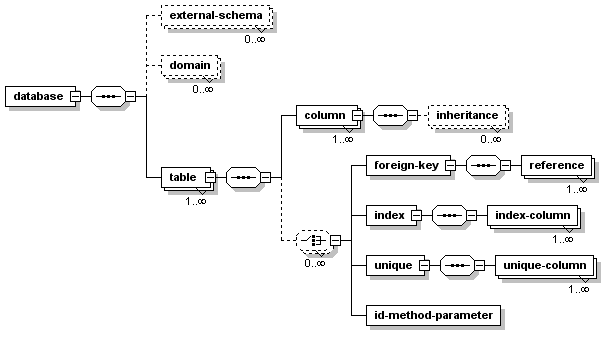
\includegraphics[height=8cm]{img/xml-config.png}
	\end{center}
	
	El esquema de base de datos de torque describe los elementos y atributos de la propia base de datos que estemos utillizando. A continuación se describe los principales elementos y las bases de datos compatibles actualmente.

Elemento: database

Puede contener los siguientes 8 atributos:

name: el nombre de la base de datos.
defaultIdMethod: este se aplica a aquellas tablas que no tienen un atributo id definido. Por defecto es “none”. Normalmente se utiliza si no quieres ID’s generados.
defaultJavaType: tipo predeterminado de las columnas de la base de datos ( “object” o “primitive”, por defecto es primitive).
package: paquete base donde se generará los modelos de objetos asociados con la base de datos. Este reemplaza la propiedad “targetPackage” del archivo build.properties de Torque.
baseClass: la clase base que se utilizará al generar el modelo de objetos.
basePeer: la clase peer a utilizar al generar los pares del modelo de objetos.
defaultJavaNamingMethod: este atributo determina como se convierten los nombres de las tablas y columnas en una clase Java o el nombre del método. Puede tener 3 valores diferentes:
nochange: no se realizan cambios.
underscore: se elimina el subrayado, la primera letra y después de un guión se pone la letra en mayúscula, el resto de caracteres en minúscula.
javaname: con guiones bajos, pero las letras no se convierten en minúscula.
heavyIndexing: agrega indices adicionales para columnas con varias claves primarias.

También puede contener los siguientes elementos:

Elemento: external-schema
Incluye otro archivo de esquema. Puede haber 0 o más elementos de este tipo.

<Externa del esquema
           		filename = "extext-schema.xml" />


Elemento: domain
Se utiliza para definir los atributos de las columnas.Puede haber 0 o más elementos de este tipo. 

<domain
           name="amount"
           type="NUMERIC"
           size="10"
           scale="2"
           default="0"
           description="amount domain" />

      
Elemento: table
Define las tablas y sus atributos:

\begin{lstlisting}[language=XML]
<table
	name="MY_TABLE"
	javaName="table"
	idMethod="idbroker"
	skipSql="false"
	baseClass="com.myapp.om.table.BaseClass"
	basePeer="com.myapp.om.table.BasePeer"
	javaNamingMethod="underscore"
	description="Table for Torque tests">

	<!-- column information here -->

</table>
\end{lstlisting}

El elemento table tiene los siguientes atributos asociados.

name: el nombre de la tabla que está siendo referenciada.
javaName: como se llamará esta tabla en Java.
idMethod: como s e crearán las claves primarias. Por defecto es nulo.
skipSql: valor booleano (true o false) que indica si hacer o no la generación de SQL para esta referencia.
abstract: valor booleano para generar la clase como abstracta o no.
baseClass: usado para la generación de OM Peer
basePeer: usado para la generación de OM Peer.
alias: define un alias para la tabla.
interface: especifica una interfaz que debería ser referenciada en la sección “implements” de la clase generada.
javaNamingMethod: especifica el nombre de la clase Java del correspondiente objeto OM. Este atributo reemplaza al atributo “defaultJavaNamingMehtod” del elemento de la base de datos (database).
description: se utiliza para la generación de documentación.

El elemento “table” también puede contener los siguientes elementos:

Elemento: column
Puede haber 1 o más elementos de este tipo por tabla.

\begin{lstlisting}
<column
           		name="MY_COLUMN"
           		javaName="Column"
           		primaryKey="true"
           		required="true"
           		size="4"
           		type="VARCHAR"
           		javaNamingMethod="underscore">

           		<!-- inheritance info if necessary -->
</column>
\end{lstlisting}

Contiene los siguientes atributos:
name: nombre de la columna que está siendo referenciada.
javaName: como se llamará esta columna en Java.
primaryKey: valor booleano que indica si es la clave primaria o no. (true o false)
required: indica si el valor es requerido.(true o false, por defecto es false)
type: de que tipo es la columna.
javaType: el tipo de la columna en Java.
size: cuantos carácteres o digitos van a ser almacenados.
default: valor por defecto si al insertar está vacio.
autoIncrement: si este campo tiene autoincremento no. (true o false, por defecto es false)
inheritance. Indica si tiene herencia. Puede tomar los valores “single” o “false”.

javaNamingMethod: especifica el nombre que será utilizado en la clase Java del correspondiente objeto OM. Este atributo reemplaza al atributo “defaultJavaNamingMehtod” del elemento de la base de datos (database).

description: se utiliza para la generación de documentación.


Elemento: foreing-key
Puede haber 0 o más elementos de este tipo por tabla.

\begin{lstlisting}
<foreign-key foreignTable="MY_TABLE"
         		 name="MY_TABLE_FK"
          		onUpdate="none"
         		 onDelete="none">
         		 <!-- reference info -->
</foreign-key>
\end{lstlisting}

Este elemento tiene 4 atributos:
foreignTable: el nombre de la tabla donde se encuentra la clave foránea.
name: el nombre de la clave foránea.
onUpdate: acción a realizar cuando se actualiza el valor en foreignTable.
onDelete: acción a realizar cuando se elimina el valor en foreingTable.

Elemento: index
Puede haber 0 o más elementos de este tipo por tabla.

\begin{lstlisting}
	<index name="MY_INDEX">
         		 <!-- index-column info -->
</index>
\end{lstlisting}

El elemento index tiene 1 atributo asociado:
name: el nombre del índice. 
Puede contener 1 o más elementos  del tipo:
	
Elemento: index-column

\begin{lstlisting}
<index-column name="INDEX_COLUMN"/>
\end{lstlisting}

Tiene solo un atributo: “name” que indica el nombre del índice de la columna. Este elemento no puede contener otros elementos.


\section{Uso de Apache Torque}

\section{Aplicacion}
\subsection{Esquema base datos}
\begin{lstlisting}[language=xml]
<!DOCTYPE database SYSTEM
 "http://db.apache.org/torque/dtd/database_3_3.dtd">

<database name="notas">
  <table name="usuario" description="Tabla de usuarios">
    <column
      name="usuario_id"
      required="true"
      primaryKey="true"
      type="INTEGER"
      description="Identificador de usuario"/>
    <column
      name="nick"
      required="true"
      type="VARCHAR"
      size="128"
      description="nick del usuario"/>
  </table>
  <table name="nota" description="Tabla de notas">
    <column
      name="nota_id"
      required="true"
      primaryKey="true"
      type="INTEGER"
      description="Identificador de nota"/>
    <column
      name="texto"
      required="true"
      type="VARCHAR"
      size="150"
      description="texto de la nota"/>
	<column
      name="usuario_id"
      required="true"
      type="INTEGER"
      description="Clave foranea de usuario"/>
	<foreign-key foreignTable="usuario">
      <reference
        local="usuario_id"
        foreign="usuario_id"/>
    </foreign-key>
  </table>
</database>
\end{lstlisting}

\end{document}